% =============================================================================
% HTR-Pipeline: Overall Concept / Workflow Diagram (v3 — minimal / title-only)
% -----------------------------------------------------------------------------
% v3 differences vs. v2:
%   - Every block reduced to a short main title (no internal implementation detail)
%   - CNN Stem and Register Tokens boxes are size- and baseline-aligned
%   - Core-contribution box uses a centered, evenly-aligned title
%   - Recognition branch ends simply at "CER"; explainability branch ends
%     simply at "Attention Map", then flows into "Downstream Applications"
%   - Legend removed (titles are self-explanatory at this level of detail)
%
% Compile standalone:   pdflatex htr_pipeline_diagram_v3.tex
% Requires: sample_input.png in the same directory as this .tex file.
% =============================================================================
\documentclass[tikz,border=6pt]{standalone}
\usepackage{graphicx}
\graphicspath{{./}}
\usetikzlibrary{arrows.meta, positioning, fit, backgrounds}

\begin{document}
\begin{tikzpicture}[
  font=\sffamily,
  every node/.style={align=center},
  arr/.style={-{Stealth[length=2.3mm, width=1.8mm]}, thick, draw=black!70},
  box/.style={rectangle, rounded corners=2pt, draw=black!65, line width=0.7pt,
              minimum height=1.0cm, minimum width=4.6cm, inner sep=4pt,
              font=\sffamily\bfseries\small},
  data/.style ={box, fill=black!5},
  cnn/.style  ={box, fill=blue!10, draw=blue!55!black},
  reg/.style  ={box, fill=orange!16, draw=orange!70!black},
  trans/.style={box, minimum height=1.1cm, fill=violet!10, draw=violet!55!black},
  ctc/.style  ={box, minimum width=4.0cm, fill=green!10, draw=green!45!black},
  attn/.style ={box, minimum width=4.0cm, fill=teal!10, draw=teal!65!black},
  down/.style ={box, minimum width=4.6cm, fill=purple!8, draw=purple!55!black},
  merge/.style={circle, draw=black!70, line width=0.6pt, fill=white, minimum size=6mm, font=\small},
  junction/.style={circle, fill=black!70, minimum size=1.6mm, inner sep=0pt},
]

% ---------------------------------------------------------------- main spine
\node[data, minimum height=1.55cm] (input) at (0,9.6)
  {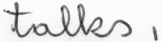
\includegraphics[width=3.2cm]{sample_input.png}\\[3pt] \textbf{Line Image}};

\node[data]  (prep)  at (0,7.85) {\textbf{Preprocessing}};

\node[reg]   (regs)  at (0,6.1)  {\textbf{Register Tokens (R)}};
\node[cnn]   (stem)  at (4.15,6.1) {\textbf{CNN Stem}};

\node[merge] (concat) at (0,4.55) {$\oplus$};
\node[trans] (transf) at (0,3.0)  {\textbf{Transformer Encoder}};

% ----------------------------------------------------- core-contribution box
\begin{scope}[on background layer]
  \node[draw=black!45, dashed, line width=0.7pt, rounded corners=4pt,
        fit=(stem)(regs)(concat)(transf), inner sep=8pt,
        label={[font=\small\sffamily\bfseries, black!55, align=center]above:Core Contribution}] (backbone) {};
\end{scope}

% -------------------------------------------------------------- arrows spine
\draw[arr] (input) -- (prep);
\draw[arr] (prep)  -- (regs);
\draw[arr] (regs)  -- (concat);
\draw[arr] (stem)  -- (concat);
\draw[arr] (concat)-- (transf);

% ------------------------------------------------------------------ branches
\node[junction] (split) at (0,1.15) {};
\draw[arr] (transf) -- (split);

\node[ctc]  (ctchead)   at (-3.15,-0.15) {\textbf{CTC Head}};
\node[attn] (aextract)  at (3.15,-0.15)  {\textbf{Attention Extraction}};
\draw[arr] (split) -| (ctchead);
\draw[arr] (split) -| (aextract);

\node[ctc]  (cer)       at (-3.15,-1.55) {\textbf{CER}};
\node[attn] (attnmap)   at (3.15,-1.55)  {\textbf{Attention Map}};
\draw[arr] (ctchead)  -- (cer);
\draw[arr] (aextract) -- (attnmap);

\node[down] (downstream) at (3.15,-2.95) {\textbf{Downstream Applications}};
\draw[arr] (attnmap) -- (downstream);

\end{tikzpicture}
\end{document}
